%----------------------------------------------------------------------------------------
%	PACKAGES AND OTHER DOCUMENT CONFIGURATIONS
%----------------------------------------------------------------------------------------

\documentclass[a4paper,12pt]{memoir} % Font and paper size

%%%%%%%%%%%%%%%%%%%%%%%%%%%%%%%%%%%%%%%%%
% Wenneker Resume/CV
% Structure Specification File
% Version 1.1 (19/6/2016)
%
% This file has been downloaded from:
% http://www.LaTeXTemplates.com
%
% Original author:
% Frits Wenneker (http://www.howtotex.com) with extensive modifications by 
% Vel (vel@latextemplates.com)
%
% License:
% CC BY-NC-SA 3.0 (http://creativecommons.org/licenses/by-nc-sa/3.0/)
%
%%%%%%%%%%%%%%%%%%%%%%%%%%%%%%%%%%%%%%%%%

%----------------------------------------------------------------------------------------
%	PACKAGES AND OTHER DOCUMENT CONFIGURATIONS
%----------------------------------------------------------------------------------------

\usepackage{XCharter} % Use the Bitstream Charter font
\usepackage[utf8]{inputenc} % Required for inputting international characters
\usepackage[T1]{fontenc} % Output font encoding for international characters

\usepackage[top=1cm,left=1cm,right=1cm,bottom=1cm]{geometry} % Modify margins

\usepackage{graphicx} % Required for figures

\usepackage{flowfram} % Required for the multi-column layout

\usepackage{url} % URLs

\usepackage[usenames,dvipsnames]{xcolor} % Required for custom colours

\usepackage{tikz} % Required for the horizontal rule

\usepackage{enumitem} % Required for modifying lists
\setlist{noitemsep,nolistsep} % Remove spacing within and around lists

\setlength{\columnsep}{\baselineskip} % Set the spacing between columns

% Define the left frame (sidebar)
\newflowframe{0.2\textwidth}{\textheight}{0pt}{0pt}[left]
\newlength{\LeftMainSep}
\setlength{\LeftMainSep}{0.2\textwidth}
\addtolength{\LeftMainSep}{1\columnsep}
 
% Small static frame for the vertical line
\newstaticframe{1.5pt}{\textheight}{\LeftMainSep}{0pt}
 
% Content of the static frame with the vertical line
\begin{staticcontents}{1}
\hfill
\tikz{\draw[loosely dotted,color=RoyalBlue,line width=1.5pt,yshift=0](0,0) -- (0,\textheight);}
\hfill\mbox{}
\end{staticcontents}
 
% Define the right frame (main body)
\addtolength{\LeftMainSep}{1.5pt}
\addtolength{\LeftMainSep}{1\columnsep}
\newflowframe{0.7\textwidth}{\textheight}{\LeftMainSep}{0pt}[main01]

\pagestyle{empty} % Disable all page numbering

\setlength{\parindent}{0pt} % Stop paragraph indentation

%----------------------------------------------------------------------------------------
%	NEW COMMANDS
%----------------------------------------------------------------------------------------

\newcommand{\userinformation}[1]{\renewcommand{\userinformation}{#1}} % Define a new command for the CV user's information that goes into the left column

\newcommand{\cvheading}[1]{{\Huge\bfseries\color{RoyalBlue} #1} \par\vspace{.6\baselineskip}} % New command for the CV heading
\newcommand{\cvsubheading}[1]{{\Large\bfseries #1} \bigbreak} % New command for the CV subheading

\newcommand{\Sep}{\vspace{1em}} % New command for the spacing between headings
\newcommand{\SmallSep}{\vspace{0.5em}} % New command for the spacing within headings

\newcommand{\aboutme}[2]{ % New command for the about me section
\textbf{\color{RoyalBlue} #1}~~#2\par\Sep
}
	
\newcommand{\CVSection}[1]{ % New command for the headings within sections
{\Large\textbf{#1}}\par
\SmallSep % Used for spacing
}

\newcommand{\CVItem}[2]{ % New command for the item descriptions
\textbf{\color{RoyalBlue} #1}\par
#2
\SmallSep % Used for spacing
}

\newcommand{\bluebullet}{\textcolor{RoyalBlue}{$\circ$}~~} % New command for the blue bullets
 % Include the file specifying document layout and packages

%----------------------------------------------------------------------------------------
%	NAME AND CONTACT INFORMATION 
%----------------------------------------------------------------------------------------

\userinformation{ % Set the content that goes into the sidebar of each page
\begin{flushright}
% Comment out this figure block if you don't want a photo
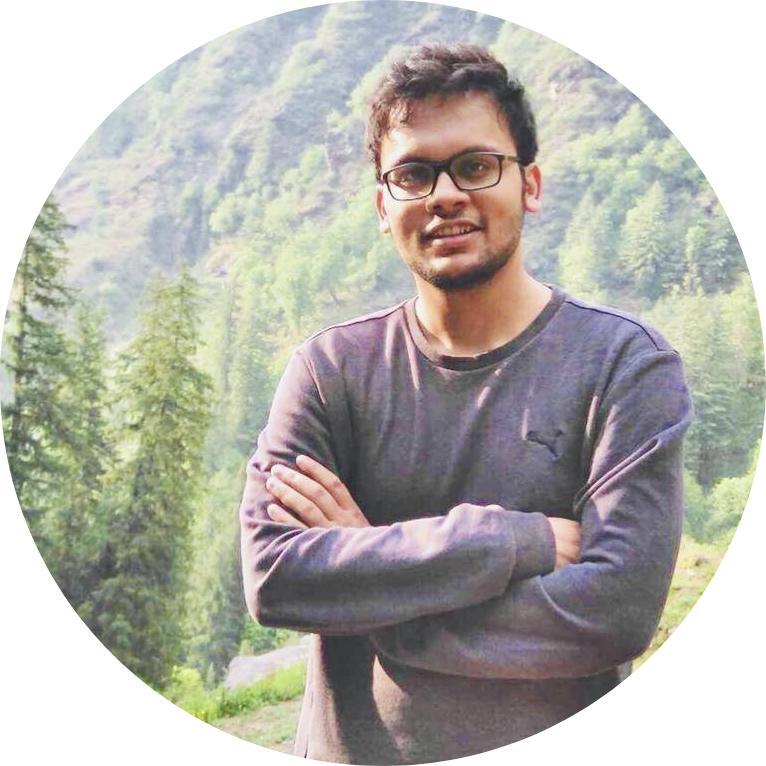
\includegraphics[width=1.1\columnwidth]{photo.png}\\[\baselineskip] % Your photo
\small % Smaller font size
\Sep % Some whitespace
\textbf{Website} \\
\url{kartikgt.github.io} \\ % Your URL
\Sep % Some whitespace
\textbf{Contact} \\
123, Society, \\ % Address 1
Bangalore, Karnatka \\ % Address 2
\vfill % Whitespace under this block to push it up under the photo
\end{flushright}
}

%----------------------------------------------------------------------------------------

\begin{document}

\userinformation % Print your information in the left column

\framebreak % End of the first column

%----------------------------------------------------------------------------------------
%	HEADING
%----------------------------------------------------------------------------------------

\cvheading{Kartik Gupta} % Large heading - your name

%\cvsubheading{Data Engineer} % Subheading - your occupation/specialization
\CVSection{Experience}
\CVItem{Jun 2018 - present, \textit{Data Engineer - IT Consultant}, SAP}{
\begin{itemize}
	\item Increased the BizX application uptime, reduced high latency jobs by 30%, and enhanced code
efficiency by providing a data discovery platform Prism to the developers and customers for real time
analytics of S2 jobs, API traffic, and ElasticAPM metrics.

	\item Built a data lake in Hadoop HDFS using Spark jobs to collect data from various sources like
Splunk, Elasticsearch, and MySQL DB, analyzed the data for business insights using Apache Hive,
and created dashboards in Kibana for visualizing the KPIs
	\item Monitored the application and automated issue resolution by creating watchers and alerts which
triggered troubleshooting python or shell scripts
	\item Managed the 25TB Hadoop cluster with 10 nodes and ensured efficient data processing of ~1
billion transactions daily including business critical jobs and APIs traffic
	\item Automated the ETL pipeline by using Jenkins and cronjobs, for reliable and real time insights
\end{itemize}
}

\CVItem{May 2017 - Jul 2017, \textit{Strategy Intern}, Nomura Finance}{
\begin{itemize}
	\item Executed a data governance project for the compliance of a broker back office data ecosystem with
the newly introduced GDPR regulations by the European Union.
\item Developed the solutions for ensuring data integrity, encryption of PIIs, and data mapping by
identifying lineages between data present in 50,000+ schemas.
\item Analyzed data for exception handling using SQL Developer and identified possible outliers.
\end{itemize}
}

\CVItem{May 2016 - Jul 2016, \textit{Consulting Intern}, Miebach Consulting}{
\begin{itemize}
	\item Identified key Indian ports and industries for targeted introduction of cold storage, CFS and ICDs to
support existing supply chain systems
	\item Designed a pilot auto replenishment system for a retail client providing automated inventory
replenishment and minimizing human errors
\end{itemize}
}

%------------------------------------------------

\Sep % Extra whitespace after the end of a major section

\CVSection{Education}
\CVItem{2013 - 2018, Indian Institute of Technology Kharagpur}{Integrated Dual Degree, Electronics and Electrical Engineering}
\Sep

\CVSection{Skills}
%\CVItem{Technical}
%{\begin{tabular}{p{0.2\textwidth} p{0.2\textwidth} p{0.2\textwidth}}
%\bluebullet Java &  \bluebullet Shell & \bluebullet Python\\
%\end{tabular}}\\

\CVItem{Technical}
{\bluebullet Led a team of 50+ to conceptualize, plan, and execute 100+ events over four days as the Events
Head at Spring Fest, the nation's biggest college socio-cultural fest with a participation of 30,00+}

\CVItem{Organizationsal}
{
\bluebullet Led a team of 50+ to conceptualize, plan, and execute 100+ events over four days as the Events
Head at Spring Fest, the nation's biggest college socio-cultural fest with a participation of 30,00+}


%------------------------------------------------
%
%\CVItem{Organizational}
%{\begin{tabular}{p{0.2\textwidth} p{0.2\textwidth} p{0.2\textwidth}}
% \bluebullet MySQL &  \bluebullet iOS & \bluebullet Android\\
%\end{tabular}}

%%------------------------------------------------
%
%\Sep % Extra whitespace after the end of a major section
%
%%----------------------------------------------------------------------------------------
%%	NEW PAGE DELIMITER
%%	Place this block wherever you would like the content of your CV to go onto the next page
%%----------------------------------------------------------------------------------------
%
%\clearpage % Start a new page
%
%\userinformation % Print your information in the left column
%
%\framebreak % End of the first column

\Sep % Extra whitespace after the end of a major section

%----------------------------------------------------------------------------------------

\end{document}
